% !TEX TS-program = xelatex
% !TEX encoding = UTF-8 Unicode

% This is a simple template for a LaTeX document using the "article" class.
% See "book", "report", "letter" for other types of document.

\documentclass[12pt]{article} % use larger type; default would be 10pt

\usepackage[utf8]{inputenc} % set input encoding (not needed with XeLaTeX)

%%% Examples of Article customizations
% These packages are optional, depending whether you want the features they provide.
% See the LaTeX Companion or other references for full information.

%%% PAGE DIMENSIONS
\usepackage{geometry} % to change the page dimensions
\geometry{a4paper} % or letterpaper (US) or a5paper or....
% \geometry{margin=2in} % for example, change the margins to 2 inches all round
% \geometry{landscape} % set up the page for landscape
%   read geometry.pdf for detailed page layout information

\usepackage{graphicx} % support the \includegraphics command and options

\usepackage[parfill]{parskip} % Activate to begin paragraphs with an empty line rather than an indent

%%% PACKAGES
\usepackage{booktabs} % for much better looking tables
\usepackage{array} % for better arrays (eg matrices) in maths
\usepackage{paralist} % very flexible & customisable lists (eg. enumerate/itemize, etc.)
\usepackage{verbatim} % adds environment for commenting out blocks of text & for better verbatim
\usepackage{subfigure} % make it possible to include more than one captioned figure/table in a single float
% These packages are all incorporated in the memoir class to one degree or another...

% \usepackage{setspace}
% \linespread{1.5}

\renewcommand{\baselinestretch}{1.2}

\usepackage{xeCJK}
\usepackage{listings}
\usepackage{xcolor}
\usepackage{float}
\usepackage{hyperref}
\usepackage{amsmath, amssymb}
\usepackage[linesnumbered,ruled]{algorithm2e}
\renewcommand{\figurename}{图}
\renewcommand{\abstractname}{摘要}
\renewcommand{\refname}{参考文献}
\hypersetup{colorlinks}

%%% HEADERS & FOOTERS
\usepackage{fancyhdr} % This should be set AFTER setting up the page geometry
\pagestyle{fancy} % options: empty , plain , fancy
\renewcommand{\headrulewidth}{0pt} % customise the layout...
\lhead{}\chead{}\rhead{}
\lfoot{}\cfoot{\thepage}\rfoot{}

%%% SECTION TITLE APPEARANCE
\usepackage{sectsty}
\allsectionsfont{\sffamily\mdseries\upshape} % (See the fntguide.pdf for font help)
% (This matches ConTeXt defaults)

%%% ToC (table of contents) APPEARANCE
\usepackage[nottoc,notlof,notlot]{tocbibind} % Put the bibliography in the ToC
\usepackage[titles,subfigure]{tocloft} % Alter the style of the Table of Contents
\renewcommand{\cftsecfont}{\rmfamily\mdseries\upshape}
\renewcommand{\cftsecpagefont}{\rmfamily\mdseries\upshape} % No bold!

%%% END Article customizations

%%% The "real" document content comes below...

\title{网络安全协议大作业}
\author{胡冬寅 \and 李锭轩 \and 林静雯}
\date{} % Activate to display a given date or no date (IF empty),
         % otherwise the current date is printed

\begin{document}
\maketitle

\section{导言}

入侵检测系统是维护系统网络安全的重要设施之一,它可以

\section{主体}
\label{main}

\subsection{应用层}
\label{app}

在计算机网络体系中,应用层的特点是种类繁多,功能多样。正是由于这种多样性,针对不同应用服务的攻击有着很大的差异,因此对它们的检测方法也是各不相同。就像应用层很难用一个协议来统一,应用层上入侵检测的方法也很难用一个比较概括的框架进行描述,因此这里仅列举几个主要的应用上的入侵检测方法。

总的来说,入侵检测的策略可以分为基于协议的检测和基于内容的检测。对于基于协议的方法,Zhang 等人根据 HTTP 错误生成模式对HTTPS协议中的恶意流量进行了检测;Manos 等人则提出了根据 NXDomian 流量来检测DNS攻击的方法。对于基于内容那个的检测,Sajjad Arshad 通过对Web网页元素进行细粒度的来源标识,达到检测基于浏览器扩展的广告注入的检测;Hugo等人则提出了一种基于发送者的邮件结构和设置信息来检测异常邮件的方案。

\subsubsection{针对协议的}
\label{protocol}

\textbf{利用NXDomian流量检测DGA}

% 逻辑上进行调整: DGA是什么 -> NXDomain流量是什么 -> 系统是怎么实现的

Manos(2017)\cite{Manos}针对基于DGA的DNS攻击,提出了根据NXDomian流量来检测恶意域名的方法。

目前,面对僵尸网络这种DNS攻击,最常见的办法是为恶意域名建立黑名单,从而过滤掉对恶意域名的查询。但攻击者利用DGA(域名生成算法)可以由一个种子制造出大量域名,使得黑名单的响应速度远远跟不上恶意域名出现的速度。人们为了应对这种攻击所使用的逆向工程方法,效果并不理想。

因此本文作者提出了根据NXDomian流量来检测恶意域名的方法。NXDomian是在用户所查询的域名无法解析时服务器产生的响应。由DGA的原理,由一个种子所产生的大量域名,只会有一小部分被注册到恶意服务器的IP地址,因此被感染的僵尸主机在查询由DGA产生的域名时必然会产生大量NXDomian流量。这个方法之所以可行,是因为由同一个DGA,同一个种子所产生的一系列域名,会有各种相同的特征。这也就是说,只要分析出由同一种子生成的NXDomain的特征,就可以利用这些特征去检测由这个种子生成的,真正被注册到恶意DNS服务器的域名了。利用这一点,作者提出了如下检测模型

\begin{figure}
	\caption{Pleiades系统示意图}
	\label{dga_pic}
	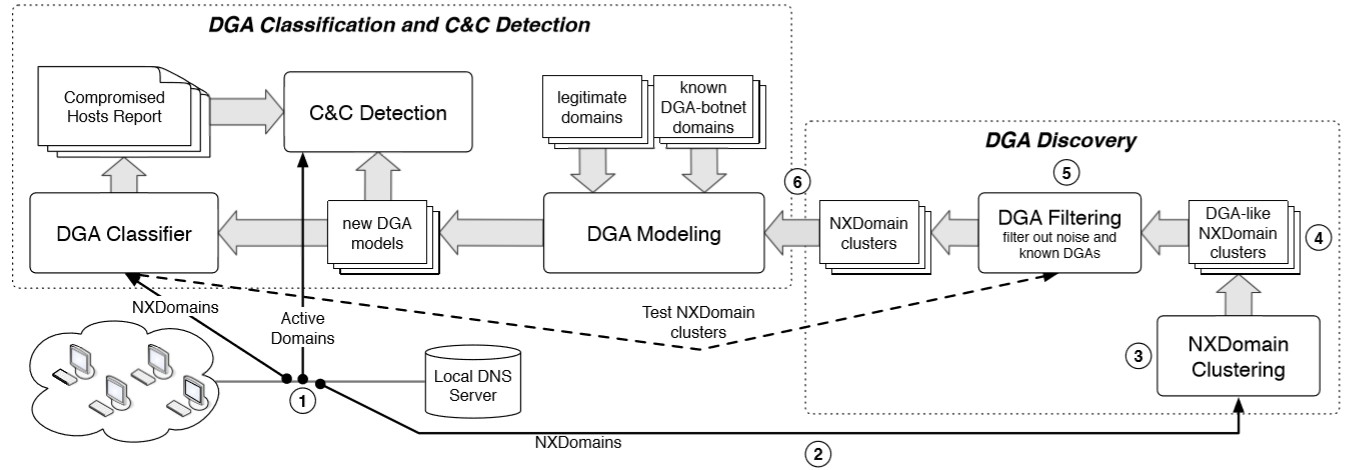
\includegraphics[width = \linewidth]{./pics/dga}
\end{figure}

此模型被部署在本地的DNS服务器。在这里,它首先会收集NXDomian流量,对这些域名送到模型中的 NXDomain Clustering 进行特征提取分析,若遇到了特征相似的一系列域名,则将它们聚合起来,并在 DGA Modeling 中与已知DGA作比较,若吻合,则将它们归类到那一种DGA中;若不吻合,则利用将这一类特征归为新的DGA,并对其建模、存储在 new DGA model 中,留待与之后收集到的域名作比较。当完成这样的工作后,由某个DGA所产生的恶意域名会大概率被检测到与某一个DGA的特征相吻合,从而可以将它列入黑名单中。

值得一提的是,NXDomian的产生并不一定是恶意的,它可能是由于用户DNS服务器配置错误,或者手误产生,如果检测提取了这种流量的特征显然是不合理的。为了避免这种情况,作者在模型中加入了一个过滤器,它可以检测出这类NXDomain,并将其过滤,利用的方法是检测域名与一些合法周知域名的相似度,若相似,则说明这类NXDomain大概率是人为失误造成,应该将其过滤。

\textbf{基于HTTP的恶意软件检测}

Zhang(2018)\cite{Zhang}等提出了良性软件和恶意软件具有不同的HTTP错误生成模式以及HTTP错误的恢复策略模式的见解,并以此作为依据设计了新的系统Error-Sensor,该系统可以仅从HTTP错误以及其附近的成功请求检测恶意软件流量。该文章主要关注的是4xx类状态码指示的HTTP错误,该类状态码用于指示的是由于客户端而导致的错误的情况。恶意软件的活动而生成的HTTP错误大多属于该类别:网络扫描攻击可能会因扫描不存在的目标404 Not Found错误,或者由于扫描受保护路径中的网页而导致403 Forbidden错误,策略违规的请求也会导致403 Forbidden错误。

并非发生HTTP错误就意味着该HTTP发起者为恶意软件,但是基于大量的现实数据,Zhang等观察到良性用户和恶意用户所生成的HTTP错误模式以及其恢复模式存在差异,该差异具体表现为,具体的表现为:受恶意软件影响的客户端通常会产生比良性客户端更多的HTTP错误,并且大多数错误都与恶意软件活动有关。并且,恶意软件生成的错误与良性用户/软件生成的错误具有显着不同的错误生成模式和恢复行为模式。存在这些不同的模式是因为良好的客户端在HTTP错误面前经常缺乏恢复例程。

\emph{Error-Sensor}检测系统就是基于这些差异来进行检测恶意软件的。在进行流量过滤以及根据客户端,服务器,网页和错误代码四元组进行错误聚类后,将错误聚类的流量进行分析,生成了错误源模式、错误生成模式、错误恢复模式这三大类特征指标,作为随机森林分类器的输入。具体来说,错误源模式包括了客户端声誉、服务端声誉、意外错误率等特征,错误生成模式包括错误生成顺序、频率等特征,错误恢复模式包括时间相关性、URI路径关联等。

结果表明,该系统在0.005\%的FPR水平下达到了99.79\%的检测率。要注意的是,该系统时DNS入侵系统的补充,因为http是在域名得到解析的前提下进行的,也就是该系统在DNS入侵系统检测失败后的进一步检测。

\textbf{基于HTTP的负载聚合技术}

Felix(2017)\cite{Felix}等提出了利用HPA载荷聚合过滤技术来识别完整的HTTP请求响应对,以减小传入到基于规则的入侵检测系统的数据量,提高性能与效率。HPA载荷聚合技术沿用了FPA和DPA的只转发每条HTTP消息的前N个字节的。经验证据表明,与入侵检测最相关的数据存储在应用层协议数据单元(PDU)的附近,而有效载荷的其余部分大多不相关,由此减少了转发到IDS中的数据量。

HPA相比于FPA和DPA的优势在于其兼容了HTTP2和HTTP1.1中所包含的流水线操作,也就是一个TCP连接中会包含多个HTTP请求-响应对。HPA的方法并不是单纯的保留每个TCP连接的每个方向的前N个字节,而是检测流水线的GET请求,以及其响应。并将GET请求以及其响应作为单个消息导出,从而允许IDS分析所有的HTTP消息的前N个字节。在评估中表明,算法HPA在仅分析2.5%的有效负载时检测到97.4%的事件。

\subsubsection{针对内容的}
\label{content}

\textbf{通过网页元素表示检测广告注入}

Sajjad Arshad(2016)\cite{Arshad}提出了一种通过细粒度的Web内容来源标识的方法来检测浏览器扩展程序插入的广告。

浏览器扩展程序很好地丰富了浏览器的功能,这为用户提供了很大的便利。但由于扩展程序一般拥有较高的权限,因此它也为攻击者提供了一个很好的平台,其中一种威胁就是基于扩展的广告注入。这种广告注入不仅可以通过播放广告来为注入者产生收益,它甚至还能使得网页发布者的合法收入转向第三方;另一方面,它可能会让用户看到不想看的内容,而用户通常不能分清这是来自第三方注入还是来自网页发布者,这给网页发布者造成了口碑上的负面影响。 % 解释一下广告注入是如何通过扩展程序实现的

为此,作者提出了\emph{ORIGINTRACER},这是一种可以集成到浏览器中的插件,它可以在文档对象模型(DOM)的粒度上标识网页元素的来源。它实现的原理是利用\textbf{起源标签集}为网页中的DOM元素做注释,因为网页无论是在从发布者的服务器加载时,在按照脚本执行时,还是进行扩展时,浏览器总是可以知道添加或是修改DOM元素的主体是什么,这时候\emph{ORIGINTRACER}就可以将这些主体添加到起源标签集中,以标识DOM元素的来源。

在分清DOM元素的来源后,\emph{ORIGINTRACER}的做法是将注入的DOM元素通过高亮或是其他一些易于发现的标识的形式展现给用户,而非直接将其删除。这样做的原因是,即便是广告注入,也很难判断用户是否需要它。因此过滤的权利被保留给用户,以帮助用户做出最有利于他们的选择。

\textbf{email}

Gascon(2018)\cite{Gascon}提出了一种基于发送者的邮件结构和设置信息,使用传统机器学习模型的鱼叉式钓鱼邮件检测方法。鱼叉式钓鱼邮件攻击是指针对特定目标构造的带有恶意链接或附件的邮件攻击,使被攻击目标无法判断该邮件是否真的来自其所声称的来源。由于不同的鱼叉式钓鱼邮件攻击相差甚远,故很难被统一抵御。在实际场景中,攻击者对其假冒的发送者的了解是有限的,而这种已知信息的有限性造成的模仿的差异性是该检测方法的关键。而Gascon提出的方法可以学习不同发送者与具体文本无关的特征,如果邮件的特征与其声称的发送者特征不相匹配,则被识别为欺骗性电子邮件。

该文章将发送者的信息提取为与具体文本无关的三类特征,分别是\textbf{行为特征}、\textbf{组成特征}以及\textbf{传输特征}。行为特征是指发送者的习惯等特征,例如是否使用数字签名,附件类型和顺序等等。组成特征则是指客户端机器配置信息,例如公共头标的类型,顺序和语法。传输特征则与邮件传输路径有关,包括Received头标和顺序,以及Received头标中提供的传递协议和TLS功能。从结果可以看到,采用这些特征学习出来的不同发送者之间具有比较高的特异性(根据曼哈顿距离),说明了该特征提取是较为成功的。并且,传输特征在这三类特征中具有最大的辨别力,而且由于其涉及基础硬件设施,也最难被伪造,所以该特征在检测中是有效的。

该文章采取了k最近邻(KNN)和支持向量机(SVM)模型,所以其所需的样本量远远少于深度学习所需要的样本量。其中KNN最少只需要2个样本,SVM为5个。这十分符合该论文所研究的特定攻击的场景——在这种特定攻击中,数据量是有限的。具体来说,来自于同一发送者的信件的量不大,故采取KNN和SVM模型适合的。特别的,SVM分类器在少量可用的电子邮件中提供了更好的性能。

\subsection{网络层及传输层}
\label{ip}

网络层与传输层信息是绝大多数NIDS会应用的信息。现行网络中最流行的网络层协议是互联网协议(IP),传输层协议是传输控制协议(TCP)和用户数据协议(UDP),绝大多数的工作在网络层与传输层的NIDS都依靠这几种协议的头标内容进行分析。

按照检测方法,网络层与传输层NIDS可以大致分为两类:\textbf{基于机器学习方法的}和\textbf{基于非机器学习方法的}。由于近些年来人工智能技术的急剧发展,越来越多的NIDS使用机器学习的方法,比如Navaporn等人利用循环神经网络(RNN)进行入侵检测。但非机器学习方法也有一定新的进展,比如A. Gaurav等人使用熵和评分手段进行检测,S. Jero等人利用有限状态机发现新的攻击。本节按照NIDS采用的不同方法展开。

\subsubsection{使用ML方法的}
\label{ml}

\textbf{使用TLS证书进行检测}

I. Torroledo等人(2018)\cite{tls}首次实现了利用TLS协议的钓鱼攻击检测。由于TLS协议中数据载荷被加密,因此难以利用载荷进行检测。该方法利用TLS协议中的证书信息进行钓鱼攻击检测;作者总结了35个与TLS证书相关的特征,使用单热(One-hot)编码方案对特征进行编码。编码后,将向量输入神经网络进行学习。

神经网络由三部分并行构成,两部分是长短时记忆模型(LSTM),用来处理证书中与被颁发主体和颁发机构相关的信息;另一部分是全连接网络,用来处理从证书中提取出的35条特征。三部分的输出结果串接构成新的输入输进全连接网络,得到最终的评分。该评分标志着干网站属于恶意网站的概率。

该方法实现了94.87\%的恶意软件检测率,88.64\%的钓鱼网站检测率。但该方法有一个不足之处——对于钓鱼网站的检测率较低,这是由于钓鱼网站的证书会伪装得与真实的证书十分相近。

\textbf{使用数据报报头信息进行检测}

Chockwanich(2019)\cite{Chockwanich}实现了在不需要人工指定规则的前提下,使用深度学习算法检测网络攻击的方法。该方法只使用了报头的相关信息,并不涉及到载荷,以此保护数据隐私。在数据预处理中,先将通过tcpdump命令获得的pcap格式流量,并删除了数据包的有效负载。然后将包数据转换为流数据。流数据不同于包数据,它是其覆盖的某个通信下的数据包的统计量和基础信息的总结,包括IP地址,持续状态,历史状态以及包速度,字节速度供16个特征等等。

在该文章的方法中,使用网络流的16个元数据作为特征供神经网络训练。为了检测和对攻击方式进行分类,该文章使用了RNN, Stacked RNN, CNN进行训练,检测了DoS攻击,端口扫描,使用UDP的网络扫描,使用TCP的网络扫描,以及使用ICMP的网络扫描这五种攻击,并实现了对这些攻击的分类。同时,作为比较,将同样的数据包放到Snort系统中检测。Snort是一个基于规则的入侵检测系统,但是其使用载荷信息进行分析,并且计算的时间很长。测试结果表明,该方案在准确率和效率上均优于Snort入侵检测系统。

\subsubsection{使用非ML方法的}
\label{nonml}

\textbf{使用熵和评分方法检测}

Akshat Gaurav等人(2017)\cite{entropy}提出了一种基于熵和评分机制的层次性DDoS攻击检测方法。该方法基于这样一个观察:在DDoS攻击期间,服务器接收到的数据包头标中的源IP地址的熵会比平常要高。该方法同时解决了如何将DDoS攻击与特定时段用户的大量访问进行区分的问题。

该方法将接收到的源IP地址按照它们到预先设置好的中心值的距离进行分组。每个组的概率$p_i$由该组内的包个数$N_i$除以数据包总数$N$计算,即$p_i = \frac{N_i}{N}$,那么源IP地址的熵表示为$H = -\sum_i p_ilog_2 p_i$;分数由当前该组的概率与历史记录中的概率相除得到。如果最近一段时间内源IP的熵如果小于阈值,当前数据会被记录下来更新分数表;如果大于阈值,那说明系统目前可能遭遇DDoS攻击,但也有可能是大量用户的正常访问。为了区分这两种情况,接着计算各组的分数,如果分数高于阈值,说明发生了DDoS攻击,不然则是正常的用户访问。

该方法综合了利用熵和计分方法的优势,做到了较低的虚警率。遗憾的是作者没有提及检测的精确率,也没有提及对于DDoS攻击和大量用户访问之间区分性有多好。但这种分析的方法在一众机器学习方法之中令人耳目一新。

\textbf{检测新型DDoS攻击——目标链路泛洪攻击}

K. Sakuma等人(2017)\cite{traceroute}介绍了一种应对新型DDoS攻击——目标链路泛洪攻击(Target link flooding attack)的方法。该方法利用traceroute进行检测。目标链路泛洪攻击不直接针对目标区域发起DDoS攻击,而是对互联网中特定的链路进行攻击,从而将目标区域与其他区域隔离。

为实现这种攻击,攻击者需要对目标区域附近的网络拓扑结构进行探测。这就需要攻击者发送大量ICMP数据包,且这些包会集中在距离目标服务器若干跳的范围内。因此通过分析距离目标服务器的不同跳数ICMP数据包可以对该类型DDoS攻击进行探测。%

首先,距离目标服务器一定范围内会部署一定量的监控器,对traceroute进行记录,并将包按照距离目标服务器的跳数进行分类;总分析服务器收集各个分散的监控器的信息,计算分数。如果两个相邻时刻的分数相差超过阈值,那么就会发出攻击警报。

这种按跳数进行恩类的思想是这篇文章的亮点所在。它克服了只利用traceroute数量变化的方法的缺点,更加健壮。但是需要部署额外的探测器是一个问题,作者没有在文章中介绍探测器数目以及部署的策略对该方法的影响。

\textbf{使用有限状态机检测TCP拥塞攻击}

Samuel Jero等人(2018)\cite{fsm}提出了一种基于有限状态机的TCP拥塞攻击发现方法。该方法受基于模型的测试(MBT)和模糊测试启发,利用TCP拥塞控制中的有限状态机作为模型指导模糊测试,从而发现新的攻击方式。

首先,该方法在有限状态机中寻找所有的可能攻击路线;然后将该路线转换成实际的攻击动作与数据包。这两部分别被称作抽象攻击策略与具体攻击策略。接着,作者在虚拟网络中进行了攻击测试,以判断该具体攻击策略是否确实显著地影响了网络流量。通过对可行的攻击策略进行分类,作者总结了11种TCP拥塞攻击,其中8种是目前文献中未被报道过的。

该方法的缺点在于,目前对于攻击的分析仍需通过日志文件由人工进行,即便可以在一定程度上自动化分析一部分,约11\%的攻击方案仍需要人工分析。

\subsection{数据链路层及物理层}
\label{phy}

本节介绍了位于数据链路层和物理层的检测方法。物理层与数据链路层位于TCP/IP栈的底层,不涉及高层协议,故具有通用性,但相对缺少高层协议中的语义信息。对于位于物理层的检测,通常需要与网络层或数据链路层的包或帧的信息结合,这是由于物理层缺乏必要的语义信息,比如对于帧的划分。另外,物理层的检测通常需要运用大量的通信方面的知识,例如对信道进行建模,计算信噪比等等。

位于数据链路层的检测通常适用于无线网络、工业网络等场合。对于无线网络,由于其共享介质的原因,容易受到干扰,这也是无线安全中的一大问题。针对IEEE 802.11协议,E. Lichtman等人利用信噪比对具体协议干扰攻击进行检测。对于工业网络,由于其协议众多,难以针对不同协议进行统一的检测。Peter Schneider等使用字节流进行通用检测,是解决该问题的方法之一。

\textbf{直接利用字节流进行入侵检测}

Peter Schneider等人(2018)\cite{cyber_phy}提出了一个可对多种现场总线协议进行异常检测的实时、统一平台。该方法直接利用线路中的字节流数据进行异常检测,因此对多种上层协议有通用性。作者提出的检测方法是,将线路中的数据包按照定长进行划分,将每一个划分的字节流作为向量输入到层叠的去噪自动编码机中。其中,层叠指隐含层是多层的,去噪是指在训练时会对训练集的数据人工添加噪声,以避免过拟合。

自动编码机的架构包含编码机和解码机,训练时二者成对的被训练。损失函数定义为由解码机恢复的向量与原向量之间均方误差。对于正常的字节流,该编码机输出的向量与原始数据之间会有很小的均方误差;而对于异常数据,编码机的输出会有明显的误差。在给定阈值的情况下,只要是误差高于阈值的数据流都被判断为存在异常。

由于该方面免除了对包中协议内容的解析,其速度明显地优于需要解析信息的方法。同时,该方法可以解构成三个模块(数据获取、数据预处理以及数据分析)并行实现,因此具备了实时性的优势。

该方法实现了对较长攻击数据流的99\%检测率。不足之处是,对于较短的攻击数据流会漏检,这是来自于该方法对数据进行批处理。

\textbf{基于信噪比的干扰攻击入侵检测}

E. Lichtman(2015)\cite{Lichtman}提出了用于检测协议感知的干扰攻击的异常入侵检测框架,可被用于802.11网络。协议感知的干扰攻击是指针对于MAC或者网络层的控制信息发起的占用网络节点通信信道的拒绝服务攻击。

文章提出的方法基于一个前提——无线接收端对于包的类型是已知的,也就是说接收端可以识别关键包和非关键包。该方法在物理层检测的基础上结合了数据链路层的协议信息,对关键包与非关键包的信噪比的统计信息进行追踪。首先,统计关键包和非关键包在一定时间段内的平均信噪比,并计算两者的比值。假设协议感知干扰存在,关键包的平均信噪比就会比较低,比值也会较低,当时间趋于无穷大时,比值趋于零。故将比值低于一定阈值的场景判定为具有协议感知的干扰攻击的存在。该框架中所设计的信噪比计算以及阈值推导,运用了大量的通信知识,这是物理层检测的一大特点。

\textbf{基于802.11的欺骗与干扰检测}

Garcia-Villegas(2015)\cite{Garcia-Villegas}提出了一种针对检测作弊行为和干扰攻击的方案,该方案应用在使用IEEE 802.11协议的局域网中。在IEEE 802.11中,\textbf{干扰攻击}可以防止节点正确执行MAC协议,或者可以导致强制重复退避的帧的冲突,因此,在IEEE 802.11其他客户端的干扰信号期间总是监测到到介质忙,从而无法使用信道。而\textbf{作弊行为或者欺骗性干扰}试图修改MAC协议的约束以获得带宽增益,使得作弊节点可以快速访问媒体介质。

该方案是利用信标访问时间(BAT)来检测作弊行为和干扰攻击。BAT被定义为从信标在信标预定传送时间(TBTT)时间点产生并被放到传输序列头部开始,一直到该信标真正被传输的时间。可以证明,当不存在作弊行为或者干扰攻击时,BAT是可以预测的。具体来说,将取决于与活动站相关的物理传输因子:站的数量,传输帧的大小,物理传输速率和提供的负载。

当作弊行为和干扰攻击存在时,BAT明显大于接入点(AP)的预测值,故可以通过BAT的偏离程度来判定是否存在作弊行为和干扰攻击。其依据为,具有作弊行为的设备可能会采取降低分布式帧间间隙(DIFS)值以更快地获得共享信道的访问,或者减小退避时间选择的竞争窗口的值来更快地获得增大访问信道的概率。而这两个行为都会导致BAT的增加。对于干扰器,BAT值随着占用时间的增加而增加,随着静默时间的增加而减少。当占用时间比较大时,占用时间主导了对BAT的影响。这是无线网络中利用链路层协议检测攻击的方法。

\section{未来工作}
\label{future}

本章讨论NIDS未来可以发展的方向。虽然目前的NIDS已经能够达到十分高的准确率,但是仍存在一些固有问题:

\begin{itemize}
	\item \textbf{数据来源}:机器学习算法的训练需要大量数据,那么数据从何而来?
	\item \textbf{面向连接型网络}:随着中间节点能力的迅猛发展,未来网络有着向连接型发展的趋势;面对连接型网络,NIDS该何去何从?
	\item \textbf{协议栈各层}:当前NIDS在各层上的实现仍存在一些问题;同时层与层之间的协作应该如何实现?
	\item \textbf{NIDS检测的攻击类型}:NIDS应该如何处理未知的攻击以及蓄意构造的针对性攻击?
	\item \textbf{使用非统计方法}:机器学习或者统计的方法有其天生的弊端,结合非统计方法是否回台给我们新的启发?
\end{itemize}

此外,目前设计的NIDS还存在\textbf{实用性}的问题——随着网络流量的不断增大,NIDS采用的检测算法是否能有效应对现实中的网络流量?以下将针对这些问题进行详细讨论。

\subsection{关于数据来源}
\label{data}

对使用机器学习或者统计的方法的入侵检测系统,需要大量的数据,比如第\ref{protocol}小节中提到的DGA分析算法,它需要大量的DNS数据集作为支撑。而在论文中,作者们总是理所当然地获得了这些数据,从中提取了所需要的特征。但这些数据并不是这么容易获得的,有些甚至是受法律限制的。因此,我们认为关于何让获取入侵数据的研究是一个值得在未来研究的方向。虽然这并非直接涉及到入侵检测,但却是做好入侵检测所必不可少的铺垫性工作。

我们设想了两大研究领域,包括:

\begin{enumerate}
	\item \textbf{数据收集}

	我们如何在法律允许的前提下,有效地收集各种数据,并形成一个开放的数据库供安全工作者们使用。这不仅为在研究新型方法的人们提供了便利,让他们不需要花费太多无谓的精力在数据收集上,还使得已提出的各种受限于数据来源的方法有可能投入到实际使用中。

	\item \textbf{数据生成}

	另一方面,受到了DGA的启发,我们想到数据集除了收集之外,是否还可以通过一个算法来生成攻击数据呢?我们将之命名为攻击生成算法(AGA)。如果我们可以设计一个有良好性能的AGA,可以根据需要伪随机地生成特定攻击类型的数据,那么相关研究的数据问题就可以得到根本性的解决了。当然,生成的数据是否符合实际,是否真的随机等问题肯定是存在的,这需要我们日后的研究来逐一解决。
\end{enumerate}

\subsection{关于面向连接型网络}
\label{connect}

目前网络传输中占据主导地位的是TCP/IP协议族,因此在讨论入侵检测时,一般来说也是基于TCP/IP协议族来进行讨论的,部署检测系统或者方案时,也常常将目光放在端点处。

但随着网络节点计算、存储能力的提升,倾向连接型网络的协议,比如ATM与MPLS,可能会得到进一步的发展。因此在未来,我们应该将一部分精力分配到适应这两种网络的入侵检测系统。比如,我们可以很自然的将IDS部署在各个节点当中,并使得节点可以将它们检测到的信息进行相互交换、整合,从而获得比只在端点检测的系统更多,更全面的对网络状况的掌握。这样一来,攻击者产生的恶意流量会更加难以躲开安全系统的检测,甚至在到达客户端之前,就会在传输过程中被某个节点过滤。从安全工作者的角度来说,他们能使用的方案、策略会更加灵活多样。 % 端点?现在也可以在中间节点(路由器)上部署IDS

另一方面,由于这种网络是面向连接的,通信双方都维护了连接的状态,这样一来IP网络中一个非常严重的问题:源地址的不确定性就得到了一定程度的解决。直接地,一些典型的与源地址修改相关的攻击的威胁会大大降低,例如IP地址欺骗、DRDOS攻击等等;间接地,在有了源地址可靠这么一个安全前提之后,我们就不需要将精力太多投入到源地址的确认上,这样自然可以提出一些新的更可靠的检测方案。 % 这一段是重点

\subsection{关于协议栈各层}
\label{layer}

\textbf{1. 应用层IDS缺少统一性方案}

在本文涉及的文章中,面对DNS服务、HTTPS协议、浏览器插件广告插入以及电子邮件等,解决的方案都是特定的、针对性的。这是受应用层特性决定的:由于应用层希望为用户提供多种多样的服务,因此应用的数据格式高度分化,很难找到统一的监测方案。是否能找到一种通用性的解决方案为应用层提供更好的安全保障呢?

受到HTTPS下层的TLS协议启发,由于上层注定无法统一,因此从其下层进行处理是更好的策略。目前有许多流行的中间件,比如Google的QUIC协议,利用这些中间件为上层应用层服务提供更好的安全性是很有意义的研究方向。

是否可以设计一种能满足多种不同应用层需求的协议?它可以灵活的组装各种模块,就像IPSec中的IKE一样,可以为差异很大的不同应用提供服务;而它又可以有效地被IDS检测和分析。这种\textbf{中间件安全}引人思考。

\textbf{2. 针对数据链路层以及物理层的监测方案较少}

在寻找合适的文章过程中,一个现象是很少有针对数据链路层或物理层进行安全监测的方案。这样的检测是有益的,考虑到:

\begin{enumerate}
    \item \textbf{应对信息受限情况}

    正如Peter Schneider等人这篇文章所述,在安全检测时,有时对上层协议不能获得完全的了解和知识,一个通用性的解决方案可以处理这样的问题;同时通用性也避免了重复开发的花费。

    \item \textbf{处理上层加密情况}

    TLS被越来越多的应用所使用;IPSec也可以对数据包进行保护;但是他们有共同的特点:数据内容被加密。这虽然为用户信息安全提供了一定的保障;但是也为攻击者提供了方便——加密的数据意味着许多方法不能被利用。而直接在数据链路层或物理层展开监测可以处理加密信息的安全监测。

    \item \textbf{对下层攻击的预防}

    在安全领域中,很常见的一种攻击方法是下层攻击。虽然本层的防御体系已经十分完善,但是对于来自下层的攻击还是力有不逮。如果,攻击者直接对电磁信号进行调整或伪造,或者在链路层中对帧进行修改,都可能会使上层的防御手段失效。
\end{enumerate}

但由于数据链路层以及物理层所包含的语义信息较少,各种检测方法有时难以实现较高的准确率。但这不代表这一层上不能够或不应该进行入侵检测。

\textbf{3. 各层之间的协作}

受到深度包检测(DPI)启发,充分利用各个层之间的信息也对实现更好的入侵检测是很有帮助的。Peter Schneider等人\cite{cyber_phy}文章中所述,一些针对工业联网设备的攻击是控制逻辑上的攻击,也即其内容本身可能符合安全标准,但是多个包连续的组合会产生特定的攻击。这样的攻击,如果能通过最初对字节流的检测,然后更进一步对报文内容进行分析处理,想必可以更进一步提高准确性,并降低虚警率。

如果凭借本层信息不能完全确定,那么可以将本层的分析结果传送到上层的检测系统中,用于辅助进一步的分析。这样的协作模式可以对检测系统的提升有很大帮助。但是这同样会面里一个问题:开销的增长。面对越来越庞大的数据流,多层协作的IDS能否实时地对系统进行保护?这需要平衡协作的程度与开销,达到一个令人满意的程度。

\subsection{关于NIDS面向的攻击类型}
\label{attack}

在入侵检测中我们所研究的各个类型的攻击中往往可以分为三类,它们是\textbf{已知的攻击},\textbf{未知的攻击},\textbf{针对已有入侵检测系统的漏洞的针对性攻击}。目前在研究中最成熟的是第一种攻击,我们可以针对性的提出各种各样的方法来检测,这样对于这一种特定攻击来说,检测效果一般会非常好。但良好的针对性往往牺牲的是通用性,在面对后面两种攻击的时候,这些检测方法的效果就会大打折扣。特别是最后一种,魔高一丈的入侵者在找准漏洞后所作出的改进后的攻击,将会在最大程度上削弱检测系统的效果。从这个角度上来说,后面这两种攻击会带来更大的安全威胁。

因此如何提出一种检测方法或者检测模型,使得它可以对可能出现的未知攻击具有很好的普适性是我们值得研究的方向。比如说,当它遇到未知的数据时,能否对它进行分析建模,并加入到一个可疑数据的库中,若日后发生了相应的安全问题,则可以据此数据库进行快速响应,避免危害的进一步扩大。

当然这只是一个粗糙的思路,并不一定经得起推敲。但这仍是一个值得我们在未来研究的方向,因为若是成功开发这样的方法,带来的安全保障将不是一些特定的检测方法所能比的。

\subsection{关于使用非统计方法}
\label{nonprob}

目前的入侵检测系统的检测方法主要有\textbf{基于规则的}和\textbf{基于统计的}。随着人工智能的兴起和算力的大幅度提高,以传统机器学习和深度学习为代表的统计方法是目前研究的主流方向。基于规则的入侵检测系统的弱点在于其性能依赖于其系统中的规则数目,而规则越多,系统的处理时间越长,效率越低。同时,由于其无法识别未知攻击,所以\textbf{漏检率}比较高。

而与基于规则的入侵检测系统不同,基于统计的方法可以检测未知攻击,但是会带来比较高的\textbf{误报率}。从理论上来看,漏检率和误报率是无法同时降低的。故如何在这两者之间进行折中处理,以符合实际的使用,是需要被关注的。

受此启发,非统计学的方法也许可以做到同时降低漏检率和误报率。由于网络中的数据主要是信息流,各种行为模式皆以信息的方式呈现,引入\textbf{信息论}的知识,也是未来的方向之一。信息论已被广泛地运用于检测DoS攻击的研究中,并表现出了比其他方法更低的误报率。如何将信息论更广泛的运用于其他的攻击检测,也是值得探讨的方向。

随着网络节点计算能力的增加,网络拓扑图的信息能够更好的被传递和储存,这使得\textbf{图论}可能成为未来入侵检测的重要方法。在计算能力大幅提升的背景下,将图论和统计结合也是一大未来的方向。

此外,传统的机器学习需要大量的人工特征提取,而这有赖于人们的先验知识,虽然对比于深度学习,前期的准备工作量更大,但更有利于实现更精准的检测,也更适用于场合特定且数据量不大的攻击检测。在统计方法中,通常需要事先将大量的数据进行预处理,这些处理过程通常是基于规则的,故如何结合基于规则和基于统计的检测系统,并发挥各自的优势,也是值得探讨的。

\begin{thebibliography}{99}

\bibitem{Manos} Antonakakis, M., April, T., Bailey, M., Bernhard, M., Bursztein, E., Cochran, J., ... \& Kumar, D. (2017). Understanding the mirai botnet. In 26th {USENIX} Security Symposium ({USENIX} Security 17) (pp. 1093-1110)

\bibitem{Arshad} Arshad, S., Kharraz, A., \& Robertson, W. (2016, September). Identifying extension-based ad injection via fine-grained web content provenance. In International Symposium on Research in Attacks, Intrusions, and Defenses (pp. 415-436). Springer, Cham.

\bibitem{tls} Torroledo, I., Camacho, L. D., \& Bahnsen, A. C. (2018, October). Hunting Malicious TLS Certificates with Deep Neural Networks. In Proceedings of the 11th ACM Workshop on Artificial Intelligence and Security (pp. 64-73). ACM.

\bibitem{cyber_phy} Schneider, P., \& Böttinger, K. (2018, October). High-Performance Unsupervised Anomaly Detection for Cyber-Physical System Networks. In Proceedings of the 2018 Workshop on Cyber-Physical Systems Security and PrivaCy (pp. 1-12). ACM.

\bibitem{traceroute} Sakuma, K., Asahina, H., Haruta, S., \& Sasase, I. (2017, December). Traceroute-based target link flooding attack detection scheme by analyzing hop count to the destination. In 2017 23rd Asia-Pacific Conference on Communications (APCC) (pp. 1-6). IEEE.

\bibitem{entropy} Gaurav, A., \& Singh, A. K. (2017, May). Entropy-score: A method to detect DDoS attack and flash crowd. In 2017 2nd IEEE International Conference on Recent Trends in Electronics, Information \& Communication Technology (RTEICT) (pp. 1427-1431). IEEE.

\bibitem{fsm} Jero, S., Hoque, E., Choffnes, D., Mislove, A., \& Nita-Rotaru, C. (2018, July). Automated attack discovery in TCP congestion control using a model-guided approach. In Proceedings of NDSS.

\bibitem{Felix} Felix Erlacher, Falko Dressler, "High Performance Intrusion Detection Using HTTP-Based Payload Aggregation" Local Computer Networks (LCN) 2017 IEEE 42nd Conference on, pp. 418-425, 2017.

\bibitem{Lichtman} Lichtman, M, Reed, JH, "Anomaly‐based intrusion detection of protocol‐aware jamming." IEEE Military Communications Conference (MILCOM'15); October 26‐28, 2015;Tampa, FL, USA.

\bibitem{Garcia-Villegas} E. Garcia-Villegas, M.S. Afaqui, E. Lopez-Aguilera, "A novel cheater and jammer detection scheme for IEEE 802.11-based wireless LANs." Elsevier J Comput Netw, 86 (2015), pp. 40-56.

\bibitem{Gascon} Gascon H., Ullrich S., Stritter B., Rieck K, "Reading Between the Lines: Content-Agnostic Detection of Spear-Phishing Emails." In: Bailey M., Holz T., Stamatogiannakis M., Ioannidis S. (eds) Research in Attacks, Intrusions, and Defenses. RAID 2018. Lecture Notes in Computer Science, vol 11050. Springer, Cham

\bibitem{Chockwanich} N. Chockwanich and V. Visoottiviseth, "Intrusion Detection by Deep Learning with TensorFlow," 2019 21st International Conference on Advanced Communication Technology (ICACT), PyeongChang Kwangwoon\_Do, Korea (South), 2019, pp. 654-659.

\bibitem{Zhang}Zhang J., Jang J., Gu G., Stoecklin M.P., Hu X. (2018) Error-Sensor: Mining Information from HTTP Error Traffic for Malware Intelligence. In: Bailey M., Holz T., Stamatogiannakis M., Ioannidis S. (eds) Research in Attacks, Intrusions, and Defenses. RAID 2018. Lecture Notes in Computer Science, vol 11050. Springer, Cham

\end{thebibliography}

\end{document}
